\chapter{Introduction}
%%------ Intro -------%%
	Since 2005  
Creating controllers for high degree of freedom complex systems is essential for development of the next generation of robots.
Due to the inherent complexity and often high expense of the system, controllers must be able to be tested.



It is common place for a complex electrical mechanical system to have multiple different controllers running in tandem.  
Different controllers are needed when the system is in different states or doing different tasks.
Combining these controllers is a problem in complex system.
This problem is hard when each controller has different frequencies, timing requirements (asyncronous vs. syncronous), latency restrictions, newest state data ie smore important then older state data and most basic of all languages the controller is written in.
This is especially true for complete and complex autonomous systems.
I define a complete and complex autonomous system as an electro mechanical mechanism with high degree of freedom (DOF) that is capable of making its own decisions through the use of sensor data processed by its artificial intelligence (AI).
The combination of high DOF and the requirement for autonomy makes the work space broad and controllers complex.
The overarching question becomes; What is the control system structure for a complete and complex autonomous systems with high DOF, a multitude of sensors, AI performing high-level and low-level tasks all while keeping a stable system structure conducive to collaborative work?
Current methods of solving the problem of controller synchrony and latest state data is to keep your critical control elements in the primary control loop.
Inter-process communication (IPC) and/or network sockets to communicate between the high level and low level processes even if written in different languages.
The majority of IPC have the problem of \textit{head of line} blocking (HOL) which means you must read the older data in a buffer before you read the newest data.
In the computer science field this is not a problem because all data being intact is typically desired.  
In the field of robotics and control the most recent state data is more important to a real-time control system to act on.
This thesis shows that by expanding on the idea of multi-process controllers connected to high-speed low-latency IPC you can create a \textit{robot layer} on a computer platform that will allow low-level controllers to run in separate processes while still allowing them access to the most recent data as the priority.
The new technical idea is the \textit{robot layer}, a control layer that allows external processes to run like normal and not deal with the specifics of the given robot system.
The robot system can be replaced by a simulated system without any of the processes needing to be modified or even know of the change.
This allows more mature controllers to be easily interfaced with this system without modifying control rates or timing.
This \textit{robot layer} must be:
\begin{itemize}
\item Have a IPC latency much less then that of the robot's inherent sampling period $t_{ipc}<<T_{r}$
\item Allow for command rates much slower then the inherent sampling period $T_{slow}>>T_{r}$
\item Allow for command rates much faster then the inherent sampling period $T_{fast}<<T_{r}$
\item Allow for arbitrary command rates.
\item Allow for real-time and non-real-time controllers to command actuators
\item Allow for all processes to have access to the newest data first
\item Allow for no more then one rt time step delay between command and robot actuator retrieval
\item Commanded such that it is for an arbitrary robotic actuator.
\item Triggering for process synchronization
\item Triggering for simulator synchronization and holding
\end{itemize}
We can succeed now not only because the bleeding edge technology allows for the fast enough communication between processes with access to the latest data.

Results are measured quantitatively and qualitatively.
Data showing proper loop rates, timings, controller implementation, simulation connections etc. show the viability of the system.
User survey shows methodology is sound, useful, and practical.





My Thesis shows is that a multi-process control structure coupled with the proper timing mechanisms is conducive to answering these questions.
It is shown with physical experiments and the creation of Hubo-Ach\cite{lofaroRAM2013}; a fully functional Sim-Time and Real-Time control system for complete and complex autonomous systems.

Through experimentation I prove my control system is a viable way of controlling complete and complex autonomous system and still be conducive to collaborative work.  
A road map of how my research has taken me to my thesis is shown in Section~\ref{sec:roadmap}.
As proof of viability I show the basic structure of my system \textit{Hubo-Ach} in Section~\ref{sec:hubo-ach}.  
I give step by step examples in Section~\ref{sec:simpleExamples}.
Section~\ref{sec:simulator} shows how we can move from real-time to using a simulated version of the platform in simulation time without having to change the controller.
Section~\ref{sec:task} describes the experiment which consists of making the robot preform an advanced task that pulls together visual, kinematic, path planning and other controllers together using this one system.
The techniques used stem from my contributions in Section~\ref{sec:contributions}.
Section~\ref{sec:results} shows the results of the experiment thus show the viability of the system.
Lastly Section~\ref{sec:conclusion} discusses the results of the work and the future of this system.

Before I continue it is important to note that my work has already been validated by my pears because:
\begin{itemize}
\item It was chosen to be the primary control system for the DARPA Robotics Challenge Track-A Team DRC-Hubo, Section~\ref{sec:drc}.
\item It is being used in the NSF-MIRR project\footnote{NSF-MIRR: Major Research Infrastructure Recovery and Reinvestment (MIRR) \#CNS-0960061 sponsored by the the U.S. National Science Foundation (NSF)}.
\item It is currently being used by MIT, WPI, Purdue, Ohio State, Swarthmore College, Georgia Tech, and Drexel University.
\end{itemize}

For the remainder of this document the complete and complex autonomous systems that I will be referring to are robots.
The majority of examples given will be in reference to humanoid robotics and the Hubo2+ (KHR-4+) platform.
The Hubo platform is described in Section~\ref{sec:hubo}.







%%------ Path To Ph.D. -------%%	
	\section{Path to Thesis}\label{sec:roadmap}	
		This section provides context to the origin of the idea of a unified algorithmic framework for complex systems.

%%%%%%% Put what I wrote here
\begin{figure}[thpb]
  \centering
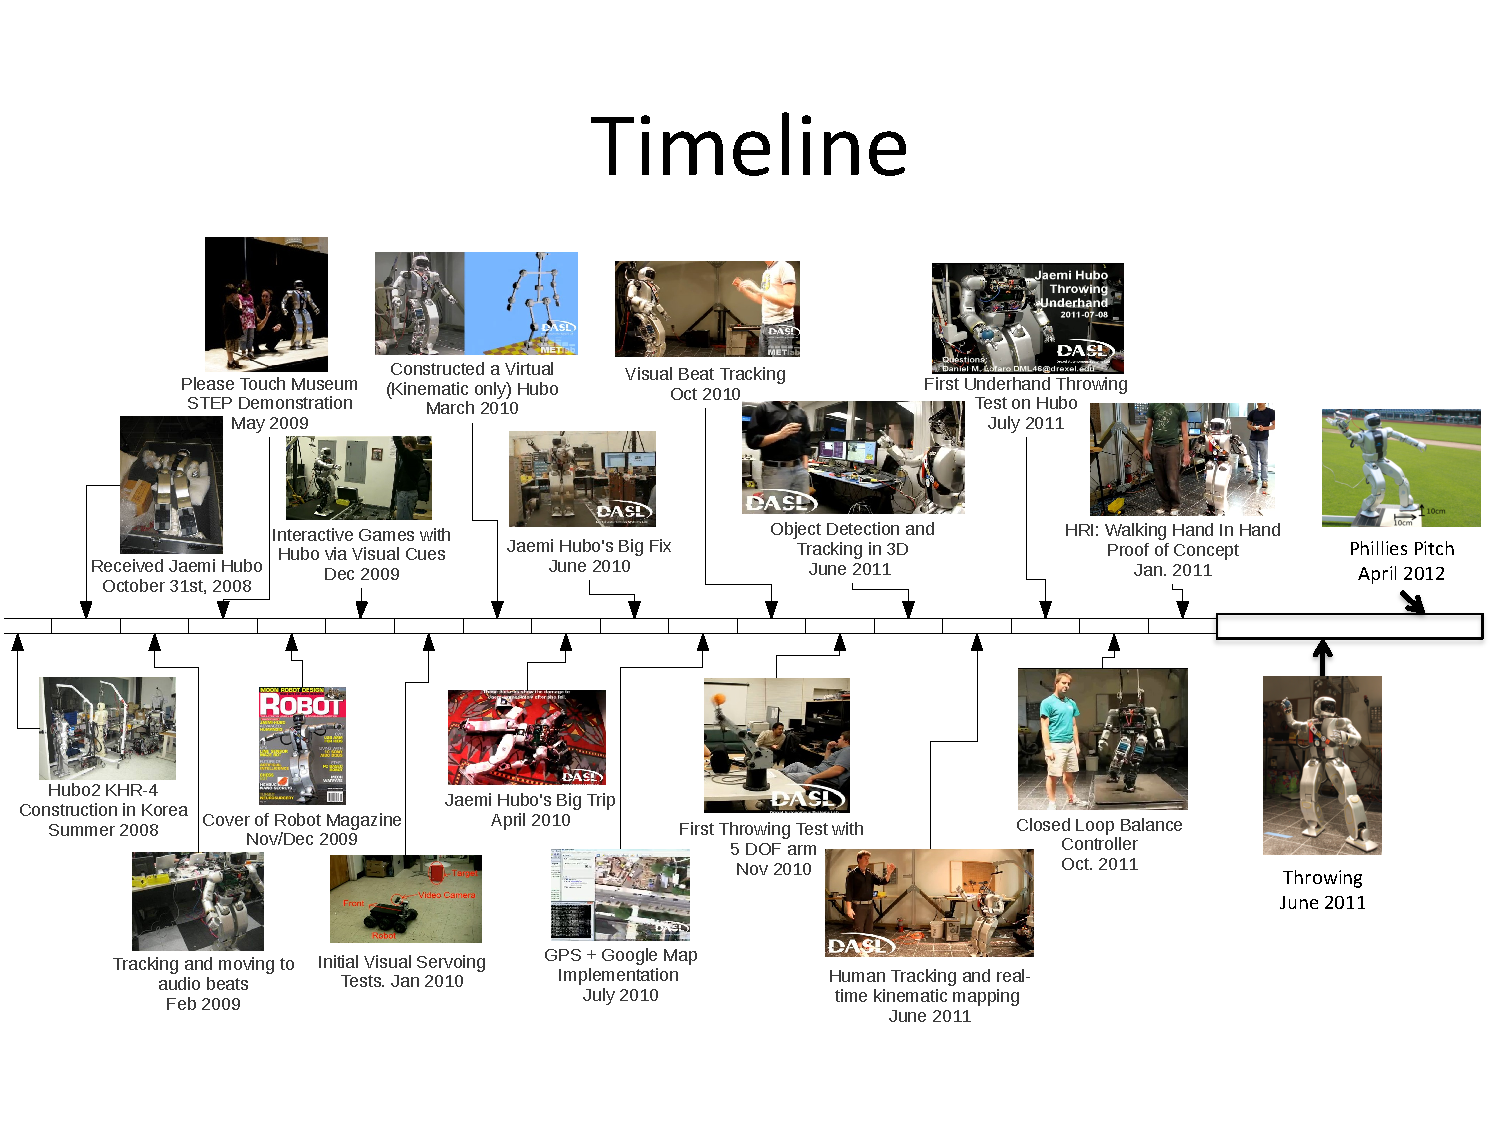
\includegraphics[angle=90, width=0.9\columnwidth]{./pix/Timeline.pdf}
  \caption{Timeline of Daniel M. Lofaro's research from 2008 to 2012}
  \label{fig:timeline}
\end{figure}

\subsection{Human Robot Interaction}
The initial goal was to have a humanoid robot become an interactive musical participant with humans.
This spawned the creation of a visual method of tracking the beat in the absence of auditory cues\cite{5686847}.
This came from a modification of a method of allowing children to play interactive games with humanoid robots\cite{lofaroGamesRobot}.
The resulting method was effective, but to increase the accuracy it was required to combine a pre-existing auditory beat tracker with the visual system.
This calumniated with a multi process system that combine the auditory and visual beat trackers\cite{lofaroIASTED2011,6094987,lofaroEURASIP2011}.
A human comparison was completed and found that this combined method was as accurate at detecting the beat in music as average humans.

\subsubsection{Results from preliminary experiments}
When collaborating with other to create a complex robot control systems integrating controllers is difficult because of the use of:
\begin{itemize}
\item different loop rates causing synchronization issues
\item different programming languages making using the same libraries a challenge
\end{itemize}

It was found that it is best to keep each working systems \textit{independent} allowing them to run at their native rate and on their native platforms\cite{ach}.



\subsection{High Degree of Freedom Kinematic Planning}
The next challenge was to perform kinematic planning for end effector velocity control. 
This resulted in the development of a method that is able to solve inverse kinematics (IK) for high degree of freedom (DOF) systems where there is no closed-form solution as well as create collision free trajectories for high DOF robots\cite{6385987}.
This is described in detail in Section~\ref{sec:srm} and \ref{sec:baseball}.
This culminated in the verification and validation of the system by an experiment where Hubo full-size humanoid robot throw the first pitch at a Major League Baseball (MLB) game\cite{lofaroHumanoids2012,6462956}.

\subsubsection{Results from preliminary experiments}
As best practice when controllers and planners are implemented it is important that low-level controllers such as balance and obstacle avoidance run at all times\cite{lofaroRAM2013}. 
Non-priority controllers such as throwing trajectory planning can run in the background in a separate process.
Keeping the processes separate allowed the system to be more resistant to lag and crashes of one or more of the controllers.
This brought validation to the overarching plan for the unified algorithmic framework for complex systems and humanoid robots.




\subsection{Lessons Learned}

At this point creating these experiment it was required to \textit{hacked} together pre-existing systems that allowed the robot to do the task.
This is the point where it was realized that a \textit{unified algorithmic framework for complex systems and humanoid robots} was required for further development in the field.
Key lessons learned from these experiments were:
\begin{itemize}
\item Must inherently decouple controllers loop rates and phases
\item Must allow for collaborators not have to \textit{inject} their code into existing source.
\item Must work with multiple robots for testing, evaluation, validation, and verification.
\end{itemize}

\noindent This is where Hubo-Ach was born.
The idea was to create a multi process architecture for humanoid control using state of the art high-speed low-latency Inter-Process Communication (IPC) techniques\cite{lofaroRAM2013}.
This is different from traditional IPC techniques because of the lack of head of line (HOL) blocking and focus on low-latency.
Section~\ref{sec:ipc} gives further details and comparisons of different IPCs.


The need for this unified framework was amplified when the Hubo was chosen to be the primary platform for the DRC-Hubo\footnote{DRC-Hubo: http://www.drc-hubo.com/} Track-A team.
Since its initial conception Hubo-Ach has become a fully functional system used in active research by multiple universities including MIT, WPI, Purdue, Ohio State, Swarthmore College, Georgia Tech, and Drexel University\cite{lofaroTePRA2013HuboAch,lofaroTePRA2013Valve}.
This research also acts as a key source of verification and validation of the system.



%%------ About Hubo -------%%
	\section{Primary Platform: Hubo2 Plus}\label{sec:hubo}
			%\subsubsection{Hubo2 Plus}
The Hubo2+ is a $1.3\meter$ (4' 3'') tall, 42 $kg$ (93 $lb$) full-size
humanoid robot.  The Hubo series was designed and constructed by the
Korean Advanced Institute of Science and Technology (KAIST) and
spinoff Rainbow Inc. \cite{hubofirst}.  It has 38 degree of freedom:
six per arm and leg, five per hand, three in the neck, and one in the
waist.  Sensors include three-axis force-torque sensors in the wrists
and ankles, accelerometers in the feet, and an inertial measurement
unit (IMU).  The sensors and embedded motor controllers are connected
via a Controller Area Network to a pair of Intel Atom PC104+ PCs
running a GNU/Linux distribution.



% The reference commands for
% all of the joints are sent from the primary control computer (x86) to
% the individual motor controllers via two Controller Area Network (CAN)
% buses.  This is the same communications bus found in most modern motor
% vehicles.  There are currently eight Hubo's functioning in the United
% States as of December 2012.  Four reside at Drexel University and one
% at Georgia Tech, Purdue, Ohio State and MIT.  Jaemi Hubo is the oldest
% of the Hubos in America and has been at the Drexel Autonomous Systems
% Lab\footnote{Drexel Autonomous Systems Lab:
%   http://dasl.mem.drexel.edu/} (DASL) since 2008 \cite{jaemiHuboSRM}.
% Fig.~\ref{fig:hubo} shows the major dimensions of Hubo.

% \begin{figure}[thpb]
%   \centering
% \includegraphics[width=1.0\columnwidth]{./pix/huboSkel.pdf}
%   \caption{Hubo2 Plus platform: 38 DOF, 130 $cm$ tall full-size humanoid robot weighing 37 $kg$.}
%   \label{fig:hubo}
% \end{figure}

% All joints of the major joints are high gain PID position
% controlled with the exception of the fingers.  The fingers are
% open-loop PWM controlled.
% The sensing capability consists of a three
% axis force-torque (FT) sensor on each leg between the end of the ankle
% and the foot as well as between the arm where it connects to the hand.
% Additionally it has an inertial measurement unit (IMU) at the center
% of mass and accelerometers on each foot.

%%% Local Variables:
%%% mode: latex
%%% TeX-master: "ach"
%%% End:

%%%                                      Sensors Chosen
%%%                                      \begin{itemize}
%%%                                      \item FT
%%%                                      \item IMU
%%%                                      \item Monocular
%%%                                      \item RGB-D
%%%                                      \end{itemize}
	%% Need to add Sensors chosen - ft, imu, monicular, stereo, rgb-d	




%%------ Inspiration -------%%	
	\section{Inspiration: DARPA Robotics Challenge}\label{sec:drc}
    	In July 2012 DARPA released a solicitation for proposals to compeat in the DARPA Robotics Challenge (DRC).
The DRC is a challenge that is in direct response to the Tsuanmi in Psuicima in 2010 (check this).
The challenge is to have a robot be able to use human tools, human vehicles and proform human tasks in an un-structured un modified human enviroment.
We applied for the grant.
In October 2012 we received word that we are a Track-A team for the DRC.
This means that we are competing agains NASA, Raythion, CMU and a team from Japan.
One of the keys to our team is our collaberation.
We are partnered with WPI, Georgia Tech, University of Delleware, Swarthmore, Purdue, Ohio State (check that) and RAINBOW (a company that rose from the Hubo Lab at Korea Advanced Institute of Science and Technology (KAIST)).
Each partner would be responsiable with one event.
We will then combine our efforts into one master controller that is cabiable of doing all the given tasks.
Having a multi-process system that also gives us the ability for our partners to share their controllers without having to intergrate their code.  
Controllers run indipendently.
	
    	%% Add DRC Pix	

%%------ Virtical Leap  -------%%	
    	\section{Controbutions and Vertical Leap}
		The primary contributions and vertical leap to the field is the creation of a \textit{unified algorithmic framework for high degree of freedom complex systems and humanoid robots}.
The resulting framework allows seamless integration of:
\begin{itemize}
\item Controllers running at different loop rates
\item Runs on multiple robots with no modification
\item Runs on simulated robots with no modification 
\item Inherent structure makes it more robust
\item Written in C for controller programing language interdependence (use C bindings in desired language)
\end{itemize}
The unified frame work Hubo-Ach is an Open-Source BSD licensed software allowing for open use.

The contributions of Hubo-Ach have been independently verified by external parties\cite{tepraDoor2013,tepraCut2013}.
Is has been validated by multiple IEEE publications\cite{lofaroTePRA2013HuboAch,lofaroTePRA2013Valve}, in review for a publication in the IEEE Robotics and Automation Society Magazine (RAM)\cite{lofaroRAM2013} and has been the top featured video on the IEEE Spectrum \textit{Video Friday} article on December 14$^{th}$, 2012\cite{videoFriday}.

		%% Works with other stuff


	
%%------ Outline of Document -------%%	
	\section{Document Outline} 
	%% NEED TO WRITE OUTLINE
	
%%------ Into To related Work ------%%
	%% this part of the document should include
		% Hubo-Ach
		% Throwing
		% IK
	%% it might belong just in the "Document Outline" part
			
			
			
			
			
			

	

